%!TEX root = um-thesis.tex

\chapter{Overview}

\section{Compilation}

The recommended method of typesetting is to use \texttt{latexmk} which handles acronyms via the \texttt{.latexmkrc} file.

\section{Acronyms}

Acronyms are handled via the \href{https://www.ctan.org/pkg/glossaries}{glossaries} package that automatically adds acronyms to a list of acronyms. Example: \gls{um} is located in \gls{aa}. \gls{um} is located in \gls{aa}. 

\section{Figures}

Tikz figures are pre-compiled via the \texttt{external} command. To name a figure, use the \texttt{\\tikzsetnextfilename} command.

\begin{figure}[h]
	\tikzsetnextfilename{example_picture}
	\begin{center}
	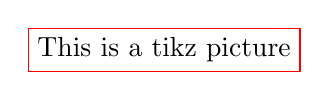
\begin{tikzpicture}
		\node[draw=red] {This is a tikz picture};
	\end{tikzpicture}
	\end{center}
	\caption{Example illustration.}
\end{figure}

\section{List of Todos}

The \href{https://www.ctan.org/pkg/todonotes}{todonotes} package is a convenient way to keep a \todo{Improve wording here}{list of todos during} the writing.  

\todo[inline, color=blue!40]{Re-read this part}

Todos can be hidden by loading the package the \texttt{disable} argument.